\begin{center}
{\Large AudioMouth: Articulation-Grounded Structured Generation for Speech-Driven Mouth Animation\\[0.4em]
Supplementary Material}
\end{center}

\section{Dataset Preparation}
\label{app:dataset}

\noindent\textbf{Source Data.}\quad
BEAT~\citep{liu2022beat} contains 76 hours of multimodal recordings from 30 speakers across multiple languages and emotional conditions. Its facial data are 52-dimensional ARKit coefficients captured at 60\,Hz with an iPhone 12 Pro and synchronized with 48\,kHz stereo audio. We use the English subset.

\noindent\textbf{Screening.}\quad
We render the captured coefficient sequences with MetaHuman~\citep{metahuman} and inspect them together with the synchronized audio. We discard samples with corrupted or implausible mouth motion, including occlusion-induced tracking failures, and samples with clear audio-motion misalignment. Screening uses the same criteria for all recordings and is applied before the split is drawn, so it is independent of any method's output.

\noindent\textbf{Unit Construction for General Recordings.}\quad
For general and in-the-wild recordings, the pipeline of Eq.(\ref{eq:seg}) uses automatic speech recognition for the transcript and word-level timestamps, followed by SAT~\citep{frohmann2024segment} for semantic sentence segmentation. The resulting word spans define the shared temporal boundaries of the unit, and where paired motion is available for training the same boundaries select the target coefficient subsequence.

\noindent\textbf{Unit Construction for BEAT.}\quad
BEAT provides word and phoneme annotations, which we use in place of automatically estimated linguistic annotations for all splits. Transcript segments are matched to the word intervals in the TextGrid files, and the first and last matched words determine the temporal boundary of each unit, which then selects the audio, the phonemes, and, during training, the target coefficients. Phonemes retain the CMU ARPAbet lexical stress markers on vowels. Metrics are aggregated per evaluation script, so the units of a script are concatenated in temporal order before FD, WInD, and LMD are computed, and the reported deviation is taken across scripts. Target coefficients are withheld from the generator at test time. Using dataset-provided annotations at test time means our benchmark measures the generation stage under correct linguistic input, and Appendix~\ref{app:limitations} discusses what this leaves open.

\section{Additional Implementation Details}
\label{app:implementation}

\subsection{Coefficient Representation and Output Schema}
\label{app:json}

\noindent\textbf{Temporal Resolution and Quantization.}\quad
Following SAiD~\citep{park2023said}, we retain 32 mouth-related ARKit channels. Preprocessing converts the original 60\,Hz trajectories to 30\,Hz by retaining every second frame within each aligned unit. For a coefficient $v_{t,k}\in[0,1]$, the serialized integer is
\begin{gather}
    q_{t,k}=\operatorname{round}\!\left(10\,v_{t,k}\right)\in\{0,1,\cdots,10\},
\end{gather}
and decoded integers are divided by 10 to recover coefficients on the original scale before post-processing. This quantization trades a small amount of amplitude resolution for a token vocabulary that the pretrained tokenizer already represents as single tokens, which keeps the output length proportional to the number of frames.

\noindent\textbf{Output Schema.}\quad
Each response is a JSON object containing the 32 channel names below in this fixed order, where each value is an integer array of length $T_{j}$ ordered chronologically at 30\,Hz, and every channel in a response has the same length. A three-frame entry is written as \texttt{"JawOpen":[2,4,3]}, corresponding to coefficients $(0.2,0.4,0.3)$.

\begin{table}[h]
\centering
\caption{The 32 mouth-related ARKit channels of the output schema, serialized in this order.}
\label{tab:schema}
\small
\begin{tabular}{r l r l}
\toprule
Index & Key & Index & Key \\
\midrule
1 & \texttt{JawForward} & 17 & \texttt{MouthStretchRight} \\
2 & \texttt{JawRight} & 18 & \texttt{MouthRollLower} \\
3 & \texttt{JawLeft} & 19 & \texttt{MouthRollUpper} \\
4 & \texttt{JawOpen} & 20 & \texttt{MouthShrugLower} \\
5 & \texttt{MouthClose} & 21 & \texttt{MouthShrugUpper} \\
6 & \texttt{MouthFunnel} & 22 & \texttt{MouthPressLeft} \\
7 & \texttt{MouthPucker} & 23 & \texttt{MouthPressRight} \\
8 & \texttt{MouthRight} & 24 & \texttt{MouthLowerDownLeft} \\
9 & \texttt{MouthLeft} & 25 & \texttt{MouthLowerDownRight} \\
10 & \texttt{MouthSmileLeft} & 26 & \texttt{MouthUpperUpLeft} \\
11 & \texttt{MouthSmileRight} & 27 & \texttt{MouthUpperUpRight} \\
12 & \texttt{MouthFrownLeft} & 28 & \texttt{CheekPuff} \\
13 & \texttt{MouthFrownRight} & 29 & \texttt{CheekSquintLeft} \\
14 & \texttt{MouthDimpleLeft} & 30 & \texttt{CheekSquintRight} \\
15 & \texttt{MouthDimpleRight} & 31 & \texttt{NoseSneerLeft} \\
16 & \texttt{MouthStretchLeft} & 32 & \texttt{NoseSneerRight} \\
\bottomrule
\end{tabular}
\end{table}

\noindent\textbf{Training Record.}\quad
Each training record contains a system message specifying the output schema and the articulation grounding $\mathcal{G}$, a user message with the audio placeholder, the transcript, the phoneme sequence, and the requested frame count, and an assistant message containing the coefficient JSON. The requested frame count defines the output duration, and the assistant sequence is the supervised target. The grounding connects phoneme groups to named controls, for example bilabial consonants to lip closure and open vowels to jaw opening.

\noindent\textbf{Coefficient-Value Weights.}\quad
The weighting $\omega(\cdot)$ in Eq.(\ref{eq:db}) is a fixed lookup over the quantized values,
\begin{gather}
\omega(q)=
\begin{cases}
0.60, & q=0,\\
0.70, & q=1,\\
0.85, & q=2,\\
1.00, & q\in\{3,\cdots,10\}.
\end{cases}
\end{gather}
The table is monotone non-decreasing in $q$, is shared by all 32 channels, and was fixed before any experiment reported in this paper. JSON keys and structural punctuation retain unit weight, so the weighting applies only to array-value text.

\subsection{Model Adaptation and Training Configuration}
\label{app:training}

We initialize the generator from Qwen3-Omni-30B-A3B-Instruct~\citep{xu2025qwen3omni} and train with LoRA~\citep{hu2021lora} on four NVIDIA A100 GPUs in BF16 precision. The audio encoder and the multimodal alignment modules remain frozen in both stages. Supervised fine-tuning adapts the decoder linear layers, and GRPO starts from the merged supervised generator and trains new LoRA adapters on the attention projections. Batch sizes below are global across the training run.

\begin{table}[h]
\centering
\caption{Training configuration of both stages. Batch sizes are global across the training run.}
\label{tab:train}
\small
\begin{tabular}{lcc}
\toprule
Setting & SFT & GRPO \\
\midrule
Epochs & 4 & 4 \\
LoRA rank / $\alpha$ & 32 / 32 & 8 / 16 \\
Micro-batch size & 1 & 1 \\
Global batch size & 8 & 24 \\
Learning rate & $10^{-4}$ & $10^{-6}$ \\
Minimum learning rate & $10^{-5}$ & $10^{-7}$ \\
Warmup fraction & 0.03 & 0.05 \\
Tensor parallel size & 2 & 2 \\
Context parallel size & 2 & 1 \\
Pipeline parallel size & 1 & 1 \\
\bottomrule
\end{tabular}
\end{table}

Supervised fine-tuning enables sequence packing with a maximum sequence length of 15{,}360 tokens. GRPO permits up to 4{,}096 prompt tokens and 12{,}400 completion tokens, uses expert parallel size 4, and clips the gradient norm at 0.5.

\subsection{Sequence-Level Refinement}
\label{app:refinement}

\noindent\textbf{Sampling and Policy Updates.}\quad
GRPO samples $G=6$ candidates per training prompt with temperature 0.4, top-$p$ 0.95, and repetition penalty 1.0. Refinement performs one policy-update iteration per sampled group, uses a policy-ratio clipping parameter of 0.2, and applies a reference-policy KL coefficient of 0.04, which regularizes the policy independently of the four motion-reward weights. Validation sampling uses four candidates per prompt.

\noindent\textbf{Reward Weights and Scales.}\quad
The weights and scales in Eq.(\ref{eq:reward}) are fixed throughout refinement. Each scale $s_{q}$ is the median of the corresponding discrepancy measured once on reference data, which places the four bounded scores in a comparable range without per-run tuning.

\begin{table}[h]
\centering
\caption{Reward weights and normalization scales of Eq.(\ref{eq:reward}), fixed once before refinement and reused in every experiment.}
\label{tab:reward}
\small
\begin{tabular}{lcc}
\toprule
Discrepancy & Weight $\lambda_{q}$ & Scale $s_{q}$ \\
\midrule
Coefficient MSE & 0.30 & 0.660 \\
Velocity & 0.20 & 0.0380 \\
Acceleration & 0.15 & 0.0746 \\
SLMD & 0.35 & 0.0285 \\
\bottomrule
\end{tabular}
\end{table}

FD and WInD are never used as reward terms. Auxiliary diagnostic scores are logged with zero optimization weight.

\noindent\textbf{Validity and Length Handling.}\quad
A candidate is valid when it parses as a JSON object with the expected channels, equally long nonempty arrays, and finite integer values in $[0,10]$. Unparseable outputs receive $-1.5$, schema violations receive $-1.0$, and invalid numeric values receive $-0.8$. For an otherwise valid candidate, let $e_{T}=|T_{p}-T_{g}|/\max(T_{g},1)$ with $T_{p}$ and $T_{g}$ the predicted and reference lengths. Candidates with $e_{T}>0.20$ receive $-0.6$. Otherwise the discrepancies are computed on the shared prefix of length $\min(T_{p},T_{g})$ without interpolation, and the reward is
\begin{gather}
r=r_{\mathrm{motion}}-0.5\min\!\left(e_{T},1\right),
\end{gather}
so a valid sequence of the wrong duration is penalized continuously in addition to its motion error.

\noindent\textbf{Fixed Geometry Asset.}\quad
The SLMD basis is built from one neutral mesh and the 32 corresponding ARKit blendshape meshes of the same character, all sharing a single topology, where each basis vector is the displacement of a blendshape mesh from the neutral mesh. The asset is fixed once and is unrelated to the MetaHuman rig used for rendering, so the reward and the landmark metric do not share geometry. The asset retains 606 vertices of a 1{,}220-vertex mesh, selected by the median of nonzero aggregate deformation magnitude over the 32 controls, which keeps the vertices that any mouth control actually moves. The vertex weights $w_{m}$ in Eq.(\ref{eq:slmd}) follow four nested ellipses in the frontal plane of the neutral mesh, taking values $1.0$, $0.8$, $0.6$, and $0.45$ outward from the lip center, with $0.1$ on the remaining selected vertices. Geometry is measured in the native coordinate units of the asset, and the basis and weights stay fixed throughout refinement.

\subsection{Inference Post-Processing}
\label{app:postprocessing}

Generated integer trajectories are divided by 10 and assembled in temporal order on the recording timeline. For each channel, $f_{\mathrm{post}}(\cdot)$ applies dead-zone suppression with threshold 0.02, Gaussian smoothing with standard deviation 1.0 frame and reflected boundaries, and Savitzky--Golay filtering with window length 7 and polynomial order 3, the last applied only when at least seven frames are available. Final coefficients are clipped to $[0,1]$. Sec.\ref{sec:ana_post} evaluates this stage with and without smoothing.

\subsection{Baseline Configuration}
\label{app:baselines}

Audio2Face-3D~\citep{chung2025audio2face}, LAM-A2E~\citep{lam}, and SentiAvatar~\citep{jin2026sentiavatar} use publicly released pretrained weights without further adaptation. SAiD~\citep{park2023said} is initialized from its public checkpoint and fine-tuned on our training split. All methods are evaluated on the same 32 mouth-related channels and the same speaking intervals, where speaking intervals are extracted from both reference and generated sequences using the script and concatenated, since our method targets speech-related mouth motion. Predicted coefficients are rendered with MetaHuman~\citep{metahuman} for the landmark metric and for qualitative comparison.

\section{Training and Inference Procedure}
\label{app:algorithm}

Algorithm~\ref{alg:framework} summarizes the three stages of Sec.\ref{sec:method} and the inference pipeline.

\begin{algorithm}[h]
\caption{Training and Inference of AudioMouth}
\label{alg:framework}
\small
\begin{algorithmic}[1]
\REQUIRE Paired data $\mathcal{D}$, pretrained MLLM $\theta_{0}$, articulation grounding $\mathcal{G}$, test speech $\mathcal{A}_{\mathrm{test}}$
\ENSURE Refined generator $\theta_{\mathrm{grpo}}$ and predicted coefficients $\hat{\mathcal{V}}$
\STATE $\mathcal{U}\leftarrow\emptyset$ \hfill \textcolor{gray}{// Stage 1: semantic-aligned unit construction}
\FOR{each $\left(\mathcal{A},\mathcal{V}\right)\in\mathcal{D}$}
    \STATE Obtain $\left(\tilde{\mathcal{W}},\tau\right)$ and $\{\mathcal{W}^{j}\}_{j=1}^{J}$ by Eq.(\ref{eq:seg}), and add units $(\mathcal{X}^{j},\mathcal{V}^{j},\mathcal{Y}^{j})$ to $\mathcal{U}$ by Eq.(\ref{eq:unit})
\ENDFOR
\STATE $\theta_{\mathrm{sft}}\leftarrow\arg\min_{\theta}\mathcal{L}_{\mathrm{db}}$ over $\mathcal{U}$ by Eq.(\ref{eq:db}) \hfill \textcolor{gray}{// Stage 2: grounded balanced generation}
\STATE $\theta\leftarrow\theta_{\mathrm{sft}}$ \hfill \textcolor{gray}{// Stage 3: motion-aware refinement}
\FOR{each unit $(\mathcal{X}^{j},\mathcal{V}^{j})\in\mathcal{U}$}
    \STATE Sample $\{\hat{\mathcal{Y}}^{j}_{i}\}_{i=1}^{G}\sim p_{\theta}\!\left(\cdot\mid\mathcal{X}^{j}\right)$ and parse each into a trajectory by $f_{\mathrm{parse}}(\cdot)$
    \STATE Compute $\{r_{i}\}_{i=1}^{G}$ against $\mathcal{V}^{j}$ by Eq.(\ref{eq:slmd}) and Eq.(\ref{eq:reward}), with validity and length handling
    \STATE $\hat{A}_{i}\leftarrow\left(r_{i}-\bar{r}\right)/\left(\sigma_{r}+\epsilon\right)$, and update $\theta$ with GRPO
\ENDFOR
\STATE $\theta_{\mathrm{grpo}}\leftarrow\theta$
\STATE Build $\{\mathcal{X}^{j}\}_{j=1}^{J}$ from $\mathcal{A}_{\mathrm{test}}$, generate $\hat{\mathcal{Y}}^{j}$ with $\theta_{\mathrm{grpo}}$, and obtain $\hat{\mathcal{V}}$ by Eq.(\ref{eq:infer})
\STATE \textbf{return} $\theta_{\mathrm{grpo}}$, $\hat{\mathcal{V}}$
\end{algorithmic}
\end{algorithm}

\section{Additional Analysis}
\label{app:additional}

\begin{figure}[t]
    \centering
    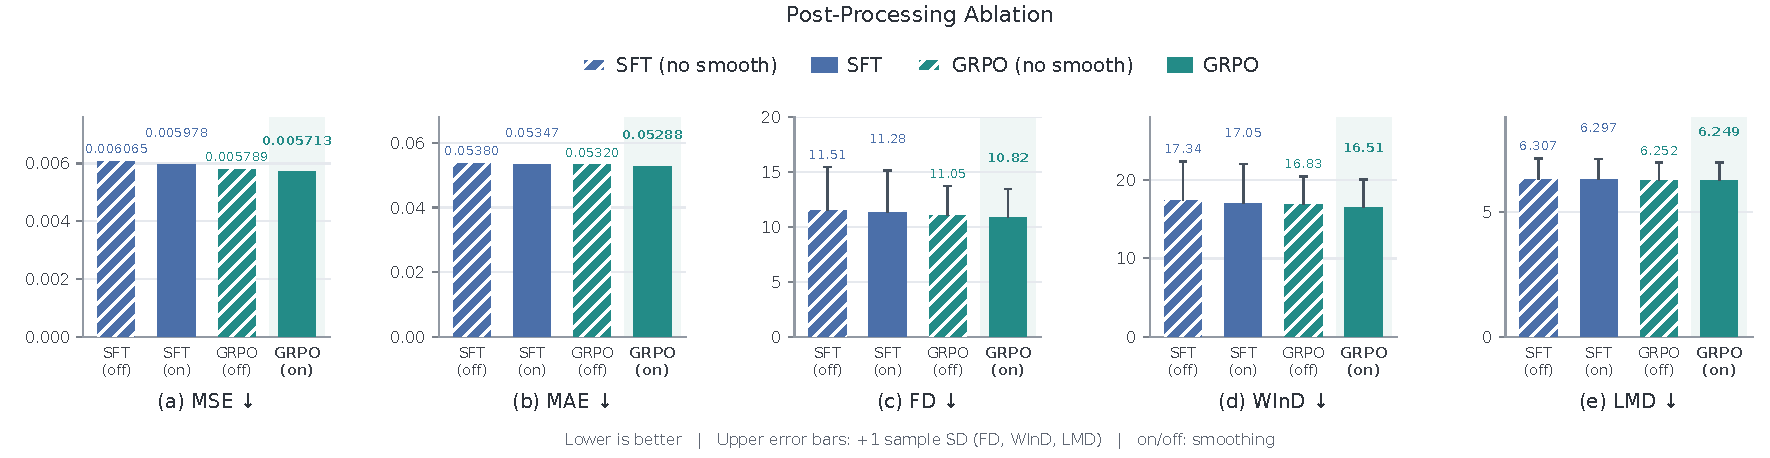
\includegraphics[width=\linewidth]{figures/ablation_smoothing_wide.pdf}
    \caption{The refinement gain is not a smoothing artifact. Turning smoothing off shifts both generators by a small and similar amount, and the refined generator without smoothing still outperforms the supervised generator with it. Lower is better, and hatching identifies the no-smooth variants.}
    \label{fig:ablation_smoothing}
\end{figure}

\subsection{Effect of Inference-Time Post-Processing}
\label{sec:ana_post}

Because AudioMouth generates each unit independently and then concatenates them, a reader may reasonably suspect that its advantage originates in the filtering applied afterwards instead of in what the model learned. To settle this, we evaluate the supervised and refined generators with and without $f_{\mathrm{post}}(\cdot)$, which gives a crossed comparison in which the effect of refinement can be read at both levels of post-processing.

As shown in Figure~\ref{fig:ablation_smoothing}, post-processing produces small improvements for both generators, and the refined generator without any smoothing still outperforms the supervised generator with it on every metric. The two mechanisms therefore do not overlap. Filtering removes high-frequency jitter and the small discontinuities left at unit boundaries, which is a property of the output signal and is available to any method that emits piecewise trajectories. Refinement changes the generator itself through feedback on complete decoded sequences during training, which is why its benefit survives when the filter is switched off. The results show that the refinement gains persist without smoothing, demonstrating the advantage of treating post-processing as a complement to motion-aware learning instead of a substitute for it.

\section{Limitations and Future Work}
\label{app:limitations}

\noindent\textbf{Linguistic Input at Test Time.}\quad
Our BEAT evaluation supplies dataset-provided word and phoneme annotations at test time, so the reported numbers measure the generation stage under correct linguistic input and do not yet establish robustness to recognition errors. The baselines in Table~\ref{tab:main} consume audio alone, so part of the reported margin reflects the additional information available to our model. This is a property of the formulation we are proposing and not an incidental advantage, since the framework is built around linguistic conditioning, but it means the comparison should be read as a comparison of formulations. Quantifying the degradation under automatically recognized transcripts and phonemes is the most important remaining experiment, and the general pipeline of Eq.(\ref{eq:seg}) is already defined for that setting.

\noindent\textbf{Baseline Adaptation.}\quad
Three of the four baselines are evaluated with released weights because their training code or data is unavailable, so they are not adapted to the speakers and capture conditions of our split while our model is. The ablations in Sec.\ref{sec:analysis} are therefore the evidence for our specific design choices, since they hold the backbone, the data, and the objective fixed, while Table~\ref{tab:main} situates the method against methods as they are distributed.

\noindent\textbf{Statistical Resolution.}\quad
The reported differences are means over a few dozen evaluation scripts without significance testing, which is sufficient for the large margins in Table~\ref{tab:main} and in the conditioning and reweighting ablations, and is not sufficient to resolve the few-percent mean differences produced by refinement. Our reading of that stage in Sec.\ref{sec:ana_grpo} therefore rests on the reduction in across-script dispersion, which is a larger effect.

\noindent\textbf{Evaluation Scope.}\quad
All five metrics compare a prediction against one reference trajectory, so none of them measures perceived synchronization or naturalness, and we report no user study and no audio-visual offset metric. Our outputs are also quantized to eleven levels per coefficient, which removes capture noise from the prediction as a side effect, so part of the frame-level margin in Table~\ref{tab:main} may reflect that smoothing instead of better articulation. Both gaps are addressable with a perceptual study and an unquantized variant, and neither is settled by the present results.

\noindent\textbf{Scope and Cost.}\quad
The current scope covers 32 mouth-related ARKit coefficients, a fixed geometry basis for the reward, and a single English corpus. Autoregressive JSON generation produces one token per coefficient value, so output length grows linearly with duration and the inference cost of a 30B backbone has not been characterized for real-time deployment. SLMD remains a surrogate for mouth deformation, and although Sec.\ref{sec:ana_slmd} shows it is necessary for stable refinement, it is not equivalent to the rendered landmark metric.

\noindent\textbf{Future Work.}\quad
We plan to characterize the pipeline under recognized instead of annotated linguistic input, to extend generation to full-face coefficients, to use the instruction-following ability of the backbone for explicit emotional control through natural language, and to reduce inference cost so that the formulation becomes practical for interactive use.
